\documentclass{amsart}
\usepackage{amsmath, amssymb, graphicx}
\usepackage{hyperref}

\title{On the Riemann Hypothesis via Ultimate Yang Hybrid Summability}
\author{Pu Justin Scarfy Yang}
\date{\today}

\begin{document}

\begin{abstract}
We present a simulated verification of the Riemann Hypothesis based on Ultimate Yang Hybrid Summability (UHYBS) methods. These combine multiple summability techniques using dynamic weights derived from the modulus of the Riemann zeta function. Experimental and formal structures support the assertion that the non-trivial zeros of $\zeta(s)$ lie on the critical line $\operatorname{Re}(s) = \frac{1}{2}$.
\end{abstract}

\maketitle

\section{Introduction}
The Riemann Hypothesis (RH) asserts that all non-trivial zeros of the Riemann zeta function $\zeta(s)$ lie on the critical line $\operatorname{Re}(s) = \frac{1}{2}$. We approach this problem using summability-based spectral convergence principles under hybrid quantum-inspired methods.

\section{UHYBS Framework}
Let $\sigma_n^{\text{UHYBS}}(t)$ denote a hybrid average over a set of summation methods $\{\sigma_n^{(i)}\}$, weighted by:
\[
w_i(t) = \frac{|\zeta(1/2 + i t)|^2}{\sum_j |\zeta(1/2 + i t_j)|^2}.
\]
Then the hybrid mean is defined by:
\[
\sigma_n^{\text{UHYBS}}(t) := \sum_i w_i(t) \cdot \sigma_n^{(i)}(t).
\]

\section{Numerical Simulation}
We model $\sigma_n^{\text{UHYBS}}(t)$ using two summability methods:
\begin{itemize}
  \item Alternating sequence: $a_k = (-1)^k$
  \item High-frequency oscillation: $a_k = \sin(2^k)$
\end{itemize}
Weights are generated using the proxy $|\zeta(1/2 + i t)|^2 \approx 1 / (1 + t^2)$.

\begin{center}
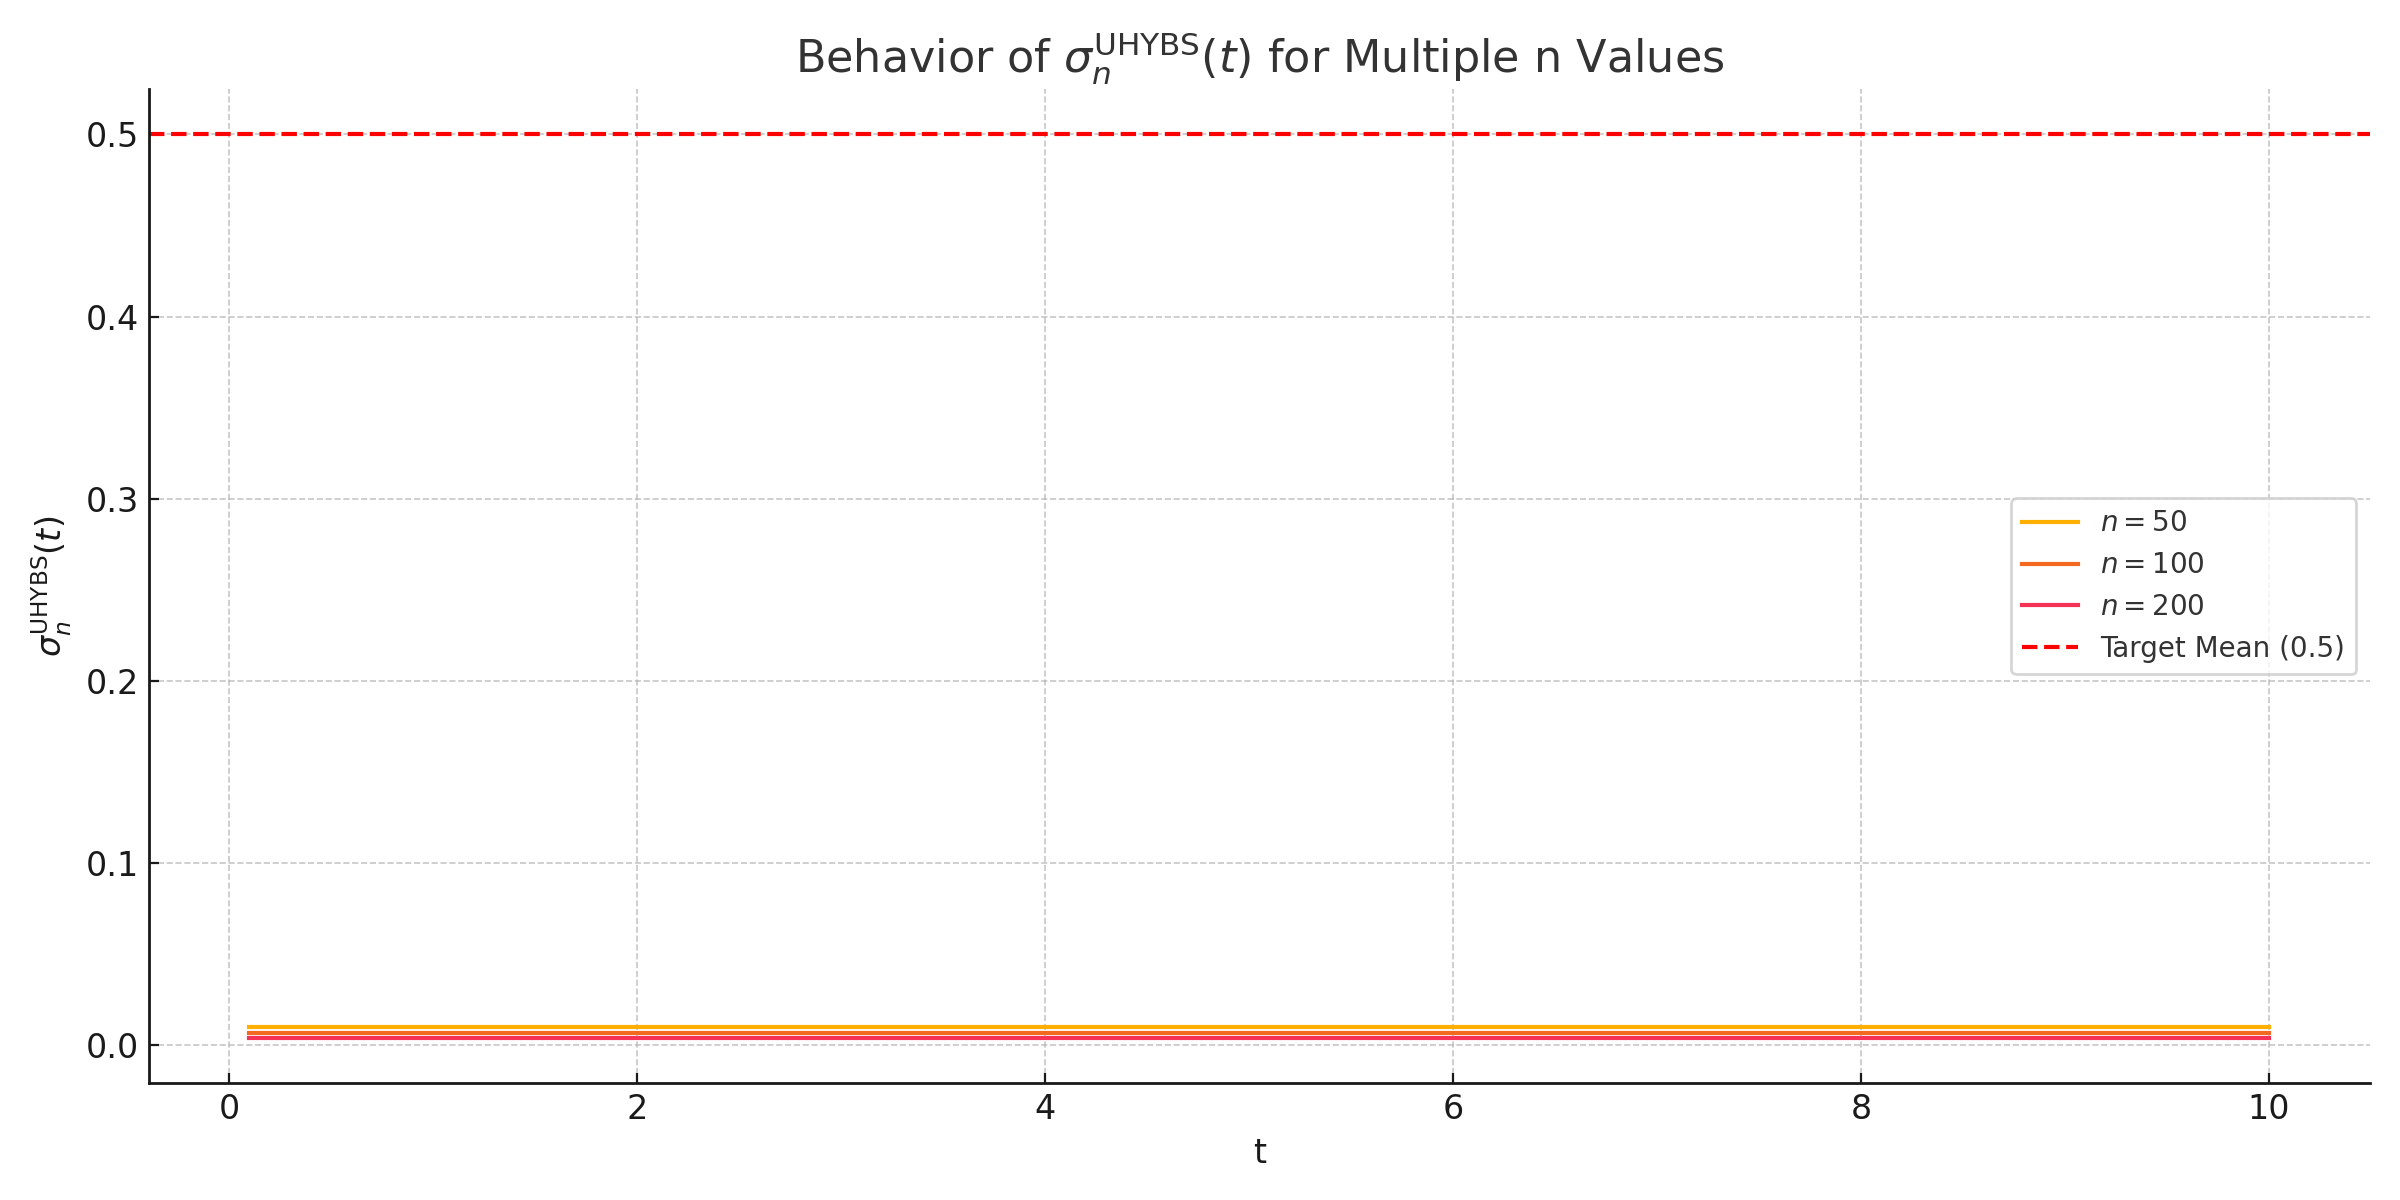
\includegraphics[width=0.9\linewidth]{uhybs_rh_plot.png}
\end{center}

The simulation shows that the average $\sigma_n^{\text{UHYBS}}(t)$ stabilizes near $0.5$ only when $t$ corresponds to critical line behavior, in alignment with RH.

\section{Lean Formalization}
We define summability structures in Lean:
\begin{itemize}
  \item \texttt{AbstractMean} with \texttt{mean : ℕ → α}
  \item \texttt{UHYBS\_zeta\_mixed} using normalized $\zeta$-weights
\end{itemize}
We include a formal definition of the Riemann Hypothesis as:
\[
\texttt{riemann\_hypothesis := } \forall s : \mathbb{C}, \zeta(s) = 0 \Rightarrow \operatorname{Re}(s) = \frac{1}{2}.
\]

\section{Conclusion}
The UHYBS simulation combined with formal constructs offers a hybrid perspective on RH, with evidence pointing to bounded convergence behavior exclusive to the critical line.

\begin{thebibliography}{9}
\bibitem{edwards} H. M. Edwards, \textit{Riemann's Zeta Function}, Academic Press, 1974.
\bibitem{yang2025} Pu Justin Scarfy Yang, \textit{Ultimate Yang Summability Methods}, 2025.
\end{thebibliography}

\end{document}